\chapter{Introduction to Continuum Mechanics}\label{ch:Collect}


This chapter starts with some historical aspects of Continuum Mechanics in order to situate the reader on the subject, which is a fundamental part of the science of Mechanics as a whole. By history of Continuum Mechanics we mean the direct contributions to the study of motion, strength and deformation of non rigid bodies; in other words, contributions to the mechanics of deformable bodies. Here, it is sufficient to rely on intuitive notions of all these concepts, which will be rigorously defined in the following chapters. Since our description is focused on non rigid bodies, works that contributed solely to the mechanics of material points will not be covered; otherwise, our history would be very, very long. Bla, bla, bla... 


\section{History}


An adequate historical account of the main contributors to the subject of Continuum Mechanics must start with the painter Leonardo da Vinci (1452-1519). Born in the city of Vinci, a comune of Florence, in the italian region of Tuscany, da Vinci became an apprentice, at the age of fourteen, in Andrea del Verrocchio's workshop, the most famous florentine artist of the time. Already informally educated on Latin, Geometry and Mathematics, at the workshop, he was taught, besides artistic abilities, a wide range of technical skills, including engineering, architecture, metallurgy and chemistry. Among his notable works, he left not only famous paintings like \emph{Mona Lisa} and \emph{The Last Supper}, but also notebooks, whose descriptive annotations and sketches cover a great variety of themes, from prosaic issues of his everyday life to exercises on Mathematics, architectural drawings, studies on painting and sculpture, engineering, cartography, astronomy, optics, botany, human anatomy, motions of fluids and solids, machine design and so on. Although it is not our purpose to criticize or profoundly analyze da Vinci's work, we must inform that in his notebooks there can be found the earliest known records on the mechanics of deformable bodies: a study on tensile test in notebook Codex Atlanticus f.222r; studies on beams and columns in notebooks Codices Atlanticus f.562r, 908r, Forster I  f.88v, 89r, Madrid I f.84v, 85v, 135v, 136r, 139r, 177v and Paris Manuscript A f.45v. Some of these records are shown in figure \ref{fg:Madrid84vAtl908r}.     
\begin{figure}[!ht]
	\centering
	\begin{center}
		\scalebox{.80}{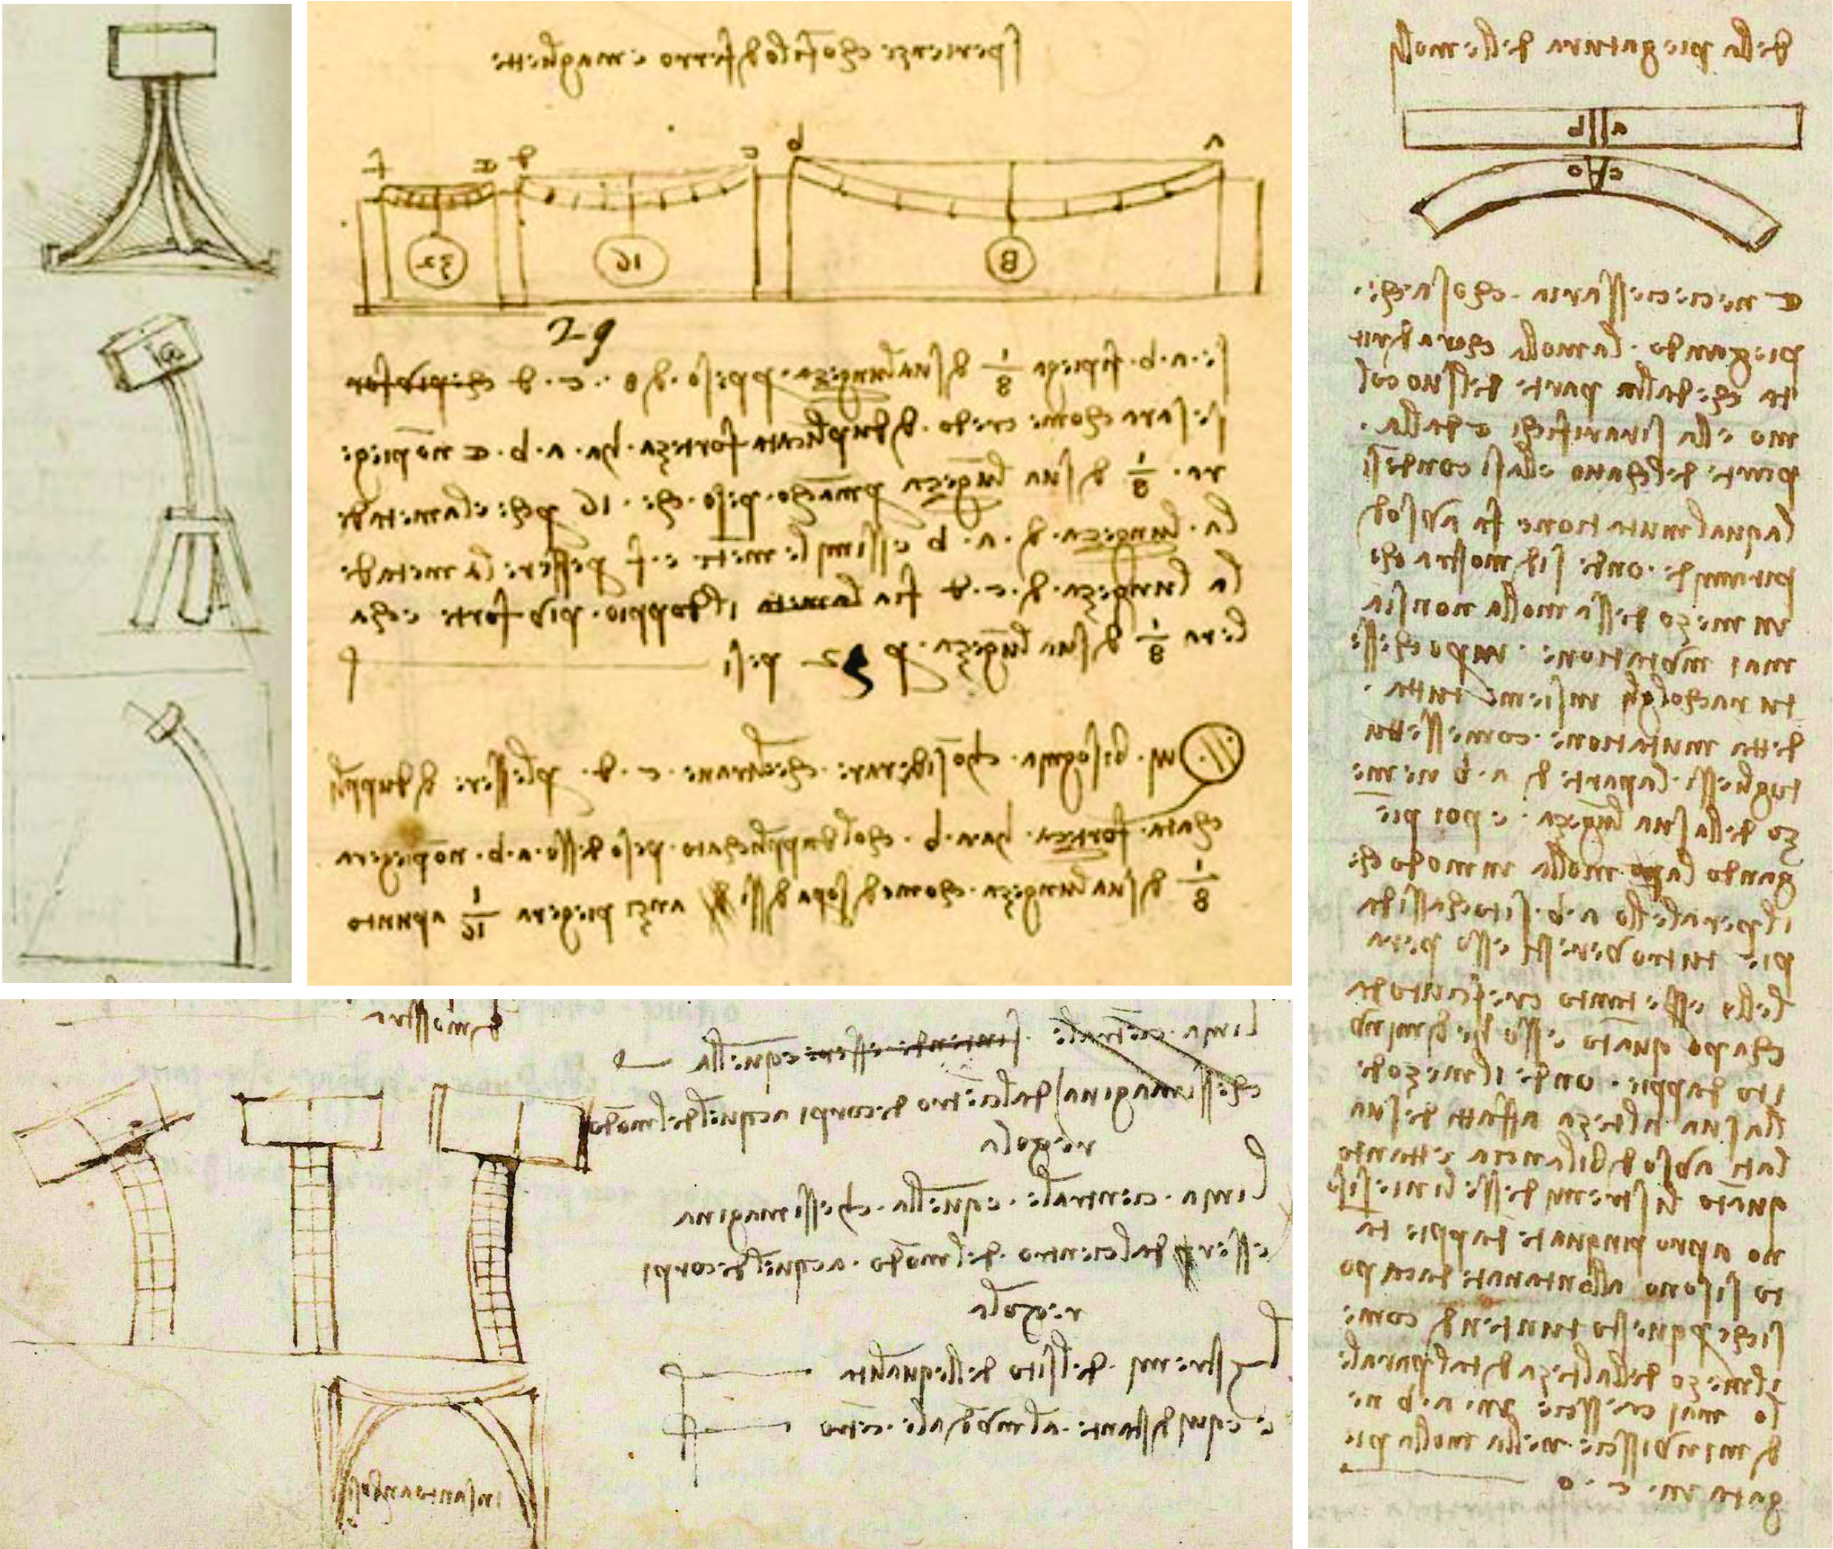
\includegraphics{partes/figs/Madrid84vAtl908r.jpg}}
	\end{center}
	\titfigura{Paris A f.45v, Atlanticus f.908r, Madrid I f.84v (right), 177v (bottom).}\label{fg:Madrid84vAtl908r}
\end{figure}
On this figure, sketches Paris A f.45v and Madrid I f.177v are studies on buckling of columns and the others are studies on bending of beams. In particular, the text on Madrid I f.84v, translated by \aut{Zammattio}\cite{zammattio_1980}, reads: \emph{``If a straight spring is bent, it is necessary that its convex part become thinner and its concave part, thicker. This modification is pyramidal, and consequently, there will never be a change in the middle of the spring. You shall discover, if you consider all of the aforementioned modifications, that by taking part 'ab' in the middle of its length and then bending the spring in a way that the two parallel lines, `a' and `b' touch a the bottom, the distance between the parallel lines has grown as much at the top as it has diminished at the bottom. Therefore, the center of its height has become much like a balance for the sides. And the ends of those lines draw as close at the bottom as much as they draw away at the top. From this you will understand why the center of the height of the parallels never increases in `ab' nor diminishes in the bent spring at `co'.''} Moreover, the striking sketch on Codex Atlanticus f.222r, entitled \emph{Testing The Strength of Iron wires of Various Lengths}, shown in figure \ref{fg:Atl222r}, is the first known record on strength of materials. 
\begin{figure}[!ht]
	\centering
	\begin{center}
		\scalebox{.75}{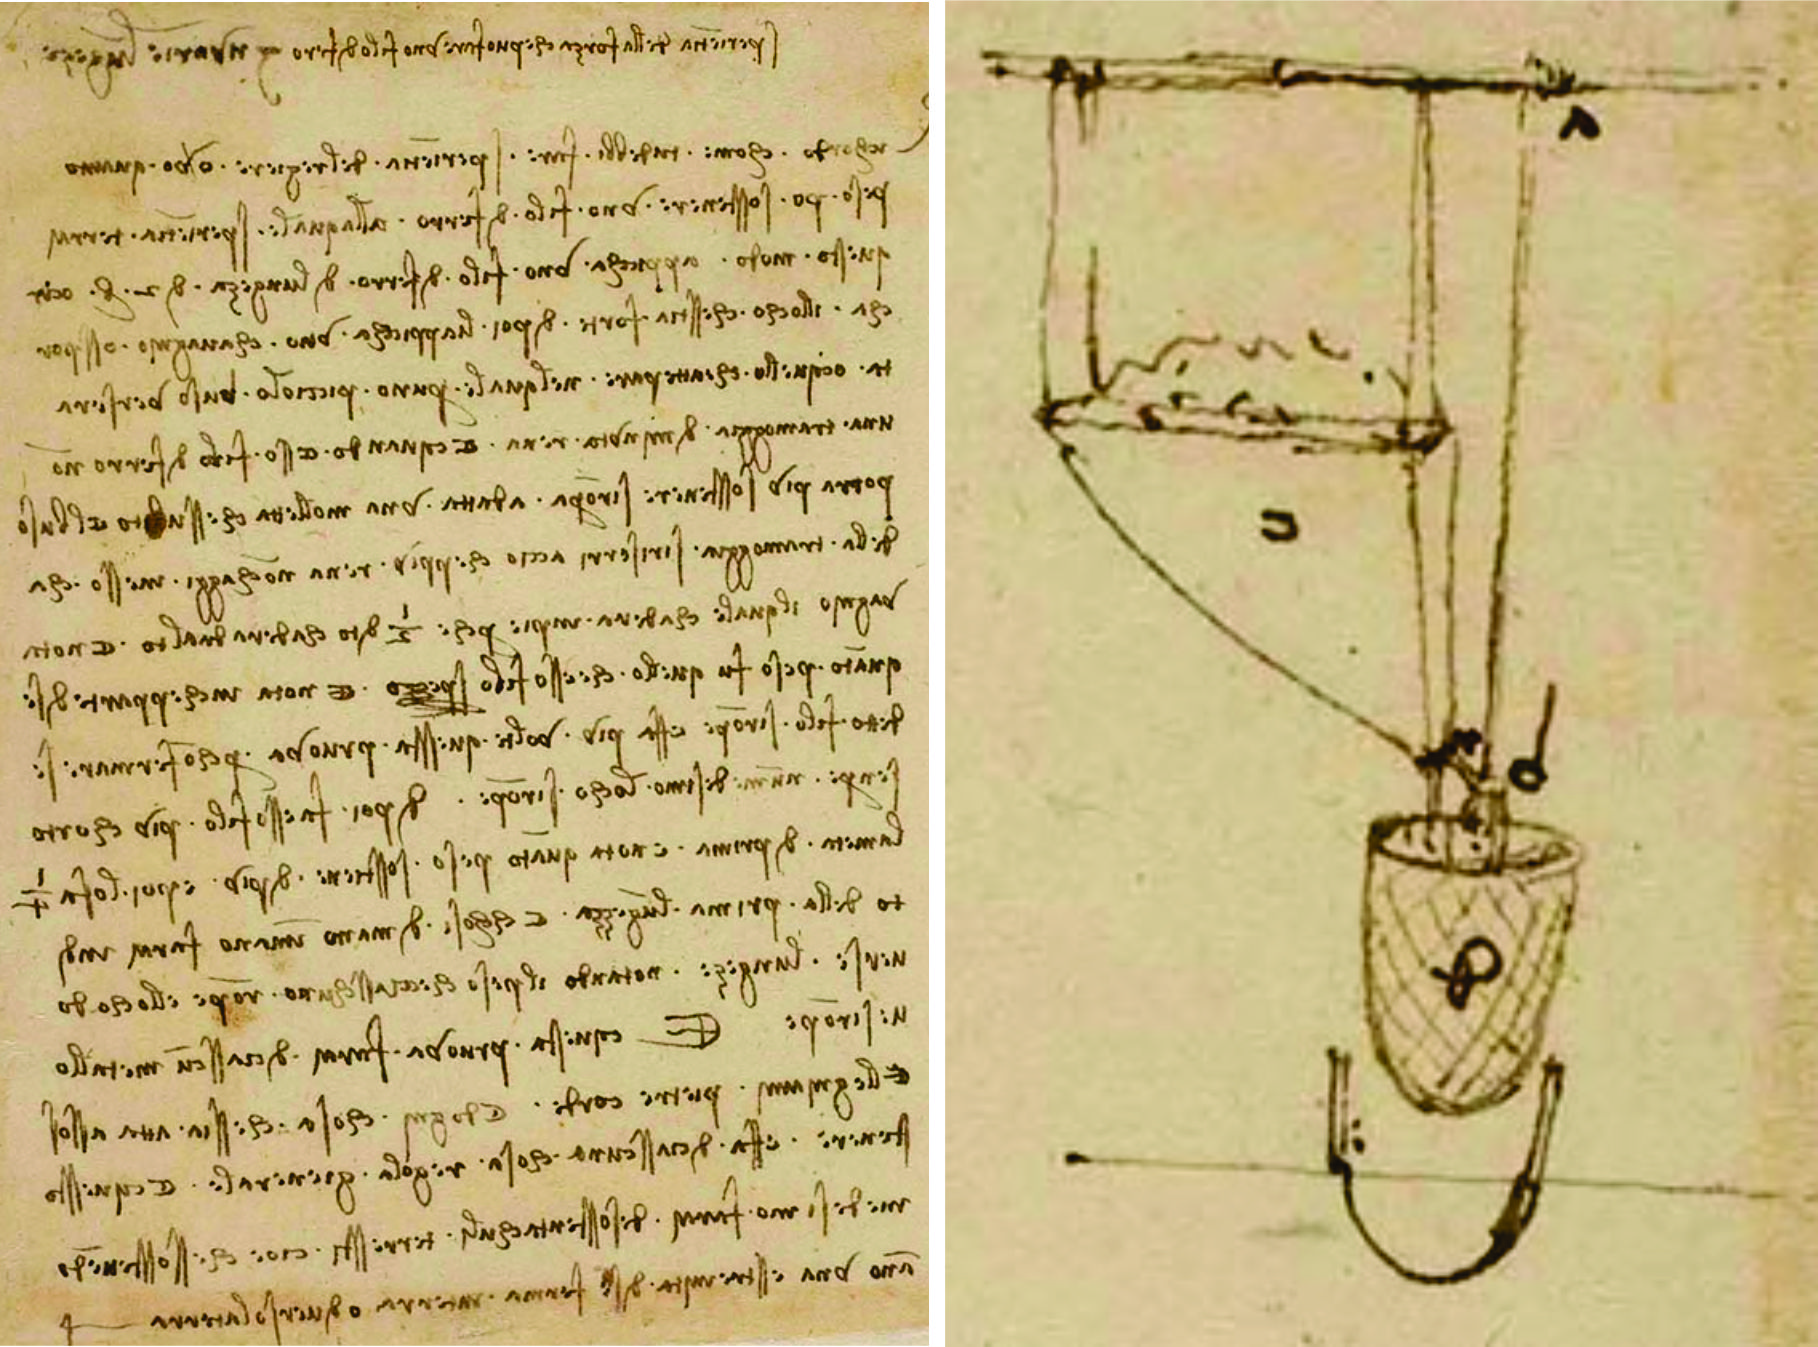
\includegraphics{partes/figs/Atl222r.jpg}}
	\end{center}
	\titfigura{Codex Atlanticus f.222r.}\label{fg:Atl222r}
\end{figure}
explicar as figuras e depois citar o texto.


Concerning Mechanics, which is our interest here, some scholars on the field contest the alleged scientific value of da Vinci's works: the most aggressive criticism is given by \aut{Truesdell}\cite{truesdell_1968}, which doubts, in his typical verbosity, whether da Vinci's sketches and annotations on engineering are really his creation or merely reproduce common technical knowledge of his time. Moreover, Truesdell says that da Vinci's proposed physical laws, all of them linear, conceived intuitively from simple rules of three, are mostly wrong and the right ones just happened to be correct, since the laws in Physics are either linear or nonlinear. According to \aut{Dugas}\cite{dugas_1988_1}, da Vinci \emph{...cuts the figure of a gifted amateur... Frequently he returned to the same problem by very different paths, and did not scruple to contradict himself}.
    